The web application, which in this case is Layer X, is the overall web portal that will be used to manage all information for any brewery products.  The web application's sole purpose is to have administrative privileges and more control of the information that is stored in the brewery's database.  Unlike the mobile application, the web portal will allow the user to add, remove, and modify any records of any brewery product that is stored in the database.

\subsection{Manage Inventory}
This section should be a general description of a particular subsystem for the given layer. For most subsystems, an extract of the architectural block diagram with data flows is useful. This should consist of the subsystem being described and those subsystems with which it communicates.

In the Manage Inventory subsystem of the web app layer, the subsystem will allow for information to be managed and stored into the brewery database.  The user will be allowed to add, delete, or modify any brewery records stored in the database by having administrative privileges for easy management of the information stored in the database.

\begin{figure}[h!]
	\centering
 	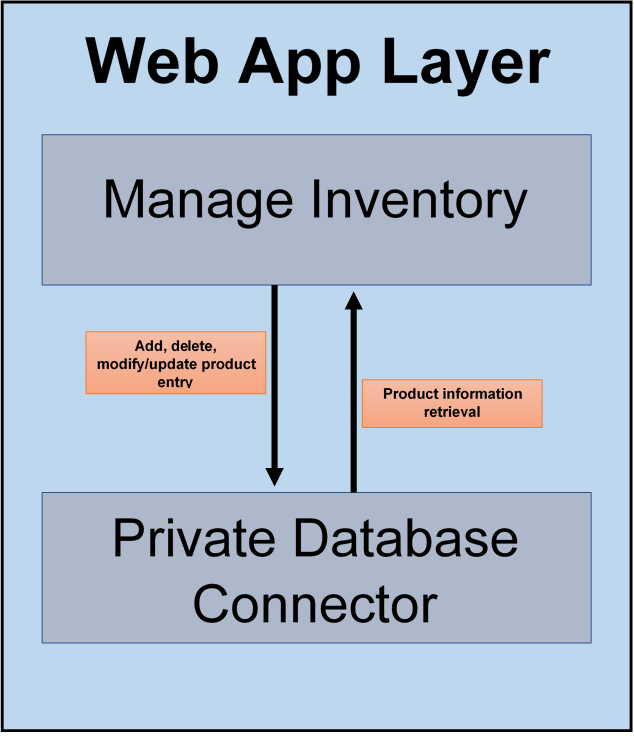
\includegraphics[width=0.60\textwidth]{images/web_app_layer.png}
 \caption{Example subsystem description diagram}
\end{figure}

\subsubsection{Assumptions}
Assuming that a brewery product is not available on the public database when the mobile app scans the barcode of the brewery product, then the web portal will allow the user to add/input the product information into the brewery database manually and become available for retrieval.  On the other hand, assuming the need for a product to be updated/modified arises, the web portal will allow the user to select the product from the database to be modified/updated and also will prompt the user which attribute of the product needs to be updated.

The Manage Inventory subsytem will interact directly with the central brewery database in the background.  Any record that is added, deleted, or modified will be stored and saved in the database once the user approves it when using the web portal.

\subsubsection{Responsibilities}
The Manage Inventory subsystem primary responsibility is for the user to interact with the user interface (UI) that'll be accessible through a web browser in order to manage any and all information stored in the central brewery database.  The user will be able to add, delete, and modify any records that are currently stored and saved on the database.  In addition, the information that'll be made available of any brewery prodcut will include the following:
Brewery
Name of beer
Style
Date of purchase
Best by date
Format (can, bottle, keg, crowler, growler, etc.)
Location (cabinet, closets, kegerator, etc.)
ID

To further explain the format and location of the brewery, the user will be able to generate a two-dimensional figure to describe the location where the products are stored physically and set the location of the brewery product in the exact row and columns of the two-dimensional figure from the cabinet, closet, kegerator, etc.

\subsubsection{Subsystem Interfaces}
Each of the inputs and outputs for the subsystem are defined here. Create a table with an entry for each labelled interface that connects to this subsystem. For each entry, describe any incoming and outgoing data elements will pass through this interface.

\begin {table}[H]
\caption {Manage Inventory Interfaces} 
\begin{center}
    \begin{tabular}{ | p{1cm} | p{6cm} | p{3cm} | p{3cm} |}
    \hline
    ID & Description & Inputs & Outputs \\ \hline
    \#01 & Web portal & \pbox{3cm}{brewery, name of beer \\ style} & \pbox{3cm}{expanded information \\ on brewery product}  \\ \hline
    \end{tabular}
\end{center}
\end{table}

\subsection{Private Database Connector}
In the Private Database Connector subsystem of the web app layer, the connector will allow a direct and secure connection to the central brewery database for information to be stored in the database layer and for information to be retrieved from the database.  The Private Database Connector will interface both with the Manage Inventory subsystem of the web portal and the central database layer.

\subsubsection{Assumptions}
The Private Database Connector will establish an interface between the web portal and the central database.  The connector will make sure that information between the web portal and the central database is exchanged accordingly.  When the web portal requests for information on a particular brewery, the connector will make the request using MySQL queries to retrieve the information from the database.  In turn, the database will receive the MySQL query and will return the information to the connector and the connector will send the information to the web portal to display it to the user.

\subsubsection{Responsibilities}
The connector's sole responsibility is to make sure that data flow between the web portal and the central database layer are well-established and for the brewery information to be securely stored and retrieved from the database.  First, the connector will establish connection to the database once it receives an input from the web portal regarding a specific brewery product.  Once the connector receives the information of the brewery product, then the connector sends the information over to the database and the database will search for the brewerey product and return additional information of the product to the connector.  The connector will then send the information to the web portal and from there the web portal will display the brewery product information to the user.
On the other hand, if the user decides to modify or delete a record from the database, the connector will send the request to the database and the database will delete or modify the record from the user's request.

\subsubsection{Private Database Connector Interfaces}
Each of the inputs and outputs for the subsystem are defined here. Create a table with an entry for each labelled interface that connects to this subsystem. For each entry, describe any incoming and outgoing data elements will pass through this interface.

\begin {table}[H]
\caption {Subsystem interfaces} 
\begin{center}
    \begin{tabular}{ | p{1cm} | p{6cm} | p{3cm} | p{3cm} |}
    \hline
    ID & Description & Inputs & Outputs \\ \hline
    \#01 & Web portal & \pbox{3cm}{brewery, name of beer \\ style} & \pbox{3cm}{expanded information \\ on brewery product}  \\ \hline
    \#02 & Central brewery DB & \pbox{3cm}{Information on \\ brewery product} & \pbox{3cm}{detailed information on product \\ sent to the connector}  \\ \hline
    \end{tabular}
\end{center}
\end{table}
